\documentclass{article}
\usepackage[utf8]{inputenc}
\usepackage{amsmath}
\usepackage{geometry}
\usepackage{graphicx}
%\usepackage{enumerate}
\usepackage{amsfonts}
\usepackage{natbib}
\usepackage{url} % not crucial - just used below for the URL 
\usepackage{cleveref}
\usepackage{float}
\usepackage[linesnumbered,ruled]{algorithm2e}
\usepackage{subfigure}
%\usepackage{lineno,hyperref} 
\usepackage{xcolor}

%\pdfminorversion=4
% NOTE: To produce blinded version, replace "0" with "1" below.
\newcommand{\blind}{0}
\let\oldref\ref
\renewcommand{\ref}[1]{(\oldref{#1})}
\DeclareMathOperator*{\argmin}{argmin}
\DeclareMathOperator*{\argmax}{argmax}


\newtheorem{prop}{Proposition}
\newtheorem{assumption}{Assumption}
\newtheorem{thm}{Theorem}
\newtheorem{proof}{Proof}


\title{Robust Boosting for Functional Regression}
%author{xmengju }
%\date{March 2021}

\begin{document}
\maketitle

\section{Methodology}
We address here the problem to estimate the regression function $F: X \rightarrow Y$, where the explanatory variable $X \in \mathcal{H}$  ($\mathcal{H}$ is a Hilbert space) and the response $Y \in \mathbb{R}$. Define the target function 
$$F = \argmin_{G}L(Y, G(x)),$$
over joint distribution of $(X,Y)$ where $L$ is a pre-specified loss function, we estimate $F$ by adapting the robust gradient boosting procedure (\texttt{RRBoost}) proposed  by \cite{ju2021robust}. 

The generalization of \texttt{RRBoost} to functional data requires using functional regressors as the base learners. A convenient choice is the type B tree adopted by our previously proposed \texttt{TFBoost}. We recall the two stage estimating procedure of \texttt{RRBoost} below and use type B trees as base learners to approximate the negative gradients in both stages:
\begin{itemize}
\item Stage 1:compute an S-type boosting estimator with high robustness but possibly low efficiency;
\item Stage 2:compute an M-type boosting estimator initialized at the function and scale estimators obtained in Stage 1.	
\end{itemize}
We call the resulted estimator \texttt{TFBoost(RR)} and outline the algorithm as follows: 

 \vspace{0.3cm}
\begin{algorithm}[H]
    \SetKwInOut{Input}{Input}
    \SetKwInOut{Output}{Output}
     \SetKwInOut{Initialize}{Initialize}
      \SetKwInOut{Stagea}{Stage 1}
     \SetKwInOut{Stageb}{Stage 2}
    \Input{A data set $(\mathbf{x}_i, y_i),  i \in \mathcal{I}_{\text{train}}$  \\
       The number of stage 1 iterations $T_1$   \\ 
       The number of stage 2 iterations $T_2$   \\ 
    The maximum depth of type B trees $d$ \\
    Breakdown point in the first stage $b$ \\
    The number of random directions of type B trees $P$ \\
    Basis $\boldsymbol{\psi} = \{\psi_1, ..., \psi_d\}$ \\
    Shrinkage parameter $\nu$ }
    \Initialize{ $\hat{F}_0(\mathbf{x})$}
     \Stagea{} 
    \hspace{1cm}   
    \For{$t = 1:T_1$}
     {
       \hspace{1cm}  $\hat{\sigma}_n (\hat{F}_{t-1}) =  \{\sigma: \frac{1}{| \mathcal{I}_{\text{train}}|}\sum_{i \in \mathcal{I}_{\text{train}}} \rho_0 \left( \frac{y_i - \hat{F}_{t-1}(x_i)}{\sigma}\right) = \kappa\}$ \\
	 \hspace{1cm}  $C_t =  \left[\sum_{i \in \mathcal{I}_{\text{train}}} \psi_0 \left(\frac{y_i - \hat{F}_{t-1}(x_i)}{\hat{\sigma}_n (\hat{F}_{t-1} )}\right) \left(\frac{y_i - \hat{F}_{t-1}(x_i)}{\hat{\sigma}_n (\hat{F}_{t-1} )}\right)\right]^{-1}$ \\
       \hspace{1cm}   $g_{t,\ell} = -C_t\psi_0 \left(\frac{y_{\ell}- \hat{F}_{t-1}(x_{\ell})} {\hat{\sigma}_n (\hat{F}_{t-1})} \right)$  \\
      \hspace{1cm}  Sample $\mathcal{P} = \{\mathbf{p}_1,..., \mathbf{p}_P\}$ \\ 
        \hspace{1cm}  $h_t = \argmin_{h \in \mathcal{H}}  \sum_{i \in |\mathcal{I}_{\text{train}}|}  \left(g_{t,i} + h\left( \mathbf{p}_1^T\langle x_i \boldsymbol{\psi} \rangle, ..., \mathbf{p}_P^T\langle x_i \boldsymbol{\psi} \rangle \right) \right)^2$ \\
       \hspace{1cm}   $\alpha_t = \argmin_{\alpha} \hat{\sigma}\left(\hat{F}_{t-1} + \alpha h_t\right)$ \\
       \hspace{1cm}   $\hat{F}_{t}(x) = \hat{F}_{t-1}(x) +  \alpha_t h_t(x)$  \\
        }
      \hspace{1cm}  $\hat{\sigma} =  \hat{\sigma}_n(\hat{F}_{T_1})$ \\
     \Stageb{}
     \hspace{1cm}
     \For{ $t = 1:T_2$}
     {
            \hspace{1cm} $g_{t,i} = - \frac{1}{\hat{\sigma}_n }
	    \psi_1 \left(\frac{y_{i}  - \hat{F}_{T_1 + t-1}(\mathbf{x}_{i})}{\hat{\sigma}_n} \right)$ \\
	        \hspace{1cm}  Sample $\mathcal{P} = \{\mathbf{p}_1,..., \mathbf{p}_P\}$ \\ 
                \hspace{1cm}  $h_t = \argmin_{h \in \mathcal{H}}  \sum_{i \in |\mathcal{I}_{\text{train}}|}  \left(g_{t,i} + h\left( \mathbf{p}_1^T\langle x_i \boldsymbol{\psi} \rangle, ..., \mathbf{p}_P^T\langle x_i \boldsymbol{\psi} \rangle \right) \right)^2$ \\
                  \hspace{1cm}  $\alpha_t = \argmin_{\alpha} \sum_{i \in \mathcal{I}_{\text{train}}} \rho_1 \left( \frac{y_i  - \hat{F}_{T_1 + t-1}(x_i)  - \alpha h_t\left( x_i \right)}{\hat{\sigma}} \right)$ \\
            \hspace{1cm} $\hat{F}_{T_1 + t}(x) = \hat{F}_{T_1 + t-1}(x) +   \alpha_t h_t(x)$ 
        }
      \Output{$\hat{F}_{T_1 + T_2}(x)$} 
          \caption{TFBoost(RR) algorithm}
            \label{code-rrboost}
\end{algorithm}


\subsection{Initialization}
\label{sec:init}
Since the loss functions involved in \texttt{TFBoost(RR)} are typically non-convex, a reliable initialization step is required to avoid reaching a local optima with a large objective value.  Especially when the breakdown point $b$ is large (close to 0.5), some ``good" initial points will have large residuals and be treated as outliers. 
To avoid this issue, we suggest using a functional multi-index tree computed with the L1 loss, which we call ``multi-index LAD tree".  This generalizes \texttt{LADTree} recommended for \texttt{RRBoost} from a multivariate setting to our functional setting.  To avoid overfitting, we use  a relatively shallow Type A tree which finds the optimal directions that minimizes the L1 prediction error.  Given projection directions $\beta_1,..., \beta_K$, we describe below the procedure to fit a Type A multi-index LAD Tree. 

Let $i \in \mathcal{I}_o$ be all the observations at a node $o$ and $R_1(j,s) = \{i| \langle x_i, \beta_j \rangle \leq s\}$ and $R_2(j,s) = \{i| \langle x_i, \beta_j \rangle > s\}$  be the left and right regions of the split made on the $j$-th index, we find $j$ and $s$ that solves
$$\min_{j\in \{1,...,P\}} \left \{\min_{s} \left(\sum_{i \in \{\mathcal{I}_o \cap R_1(j, s)\}} |y_i - \text{med}(y_i)| + \sum_{i \in \{\mathcal{I}_o \cap R_2(j, s)\}}|y_i - \text{med}(y_i)| \right) \right \}. $$
This procedure is repeated until the tree reaches the maximum depth ($d_{\text{init}}$) or minimum number of observations per node ($m_{\text{init}}$).  We denote the resulted tree $h_{\text{init}}(\langle x,\beta_1 \rangle, ...,\langle x,\beta_K \rangle )$. 


To fit a  Type A multi-index  LAD tree, we find $\beta_1,..., \beta_K$ that minimizes the L1 loss on the entire tree: 

$$\argmin_{\beta_1,..., \beta_K} \sum_{i=1}^n|y_i - h_{\text{init}}(\langle x_i,\beta_1 \rangle, ...,\langle x_i,\beta_K \rangle)|.$$

%To select the parameters ($d_{\text{init}}$ and $m_{\text{init}}$) of the initial tree, we follow the procedure below. 



%first fit \texttt{RTFBoost} using the median of the responses as the initial fit: $$\hat{F}_0(x) = \text{median}( \{y_i| i \in \mathcal{I}_{\text{train}}\}),$$
%and flagged potential outliers ($\mathcal{I}_f$) as those with residuals deviating from their median by more than 3 times their MAD. Then we fit \texttt{RTFBoost} with multi-index LAD tree for  each combination of ($d_{\text{init}}$, $m_{\text{init}}$) under consideration,  and chose the one that performs the best on the validation set, where  the performance is evaluated as the absolute deviation of residuals of non-flagged validation data points: 
%$$\sum_{i \in \mathcal{I}_{\text{val}}/\mathcal{I}_{\text{f}}} \left|y_i - \hat{F}_{T_1 + T_2}(x_i) \right|.$$


\subsection{Early stopping}
Same as what we did for \texttt{RRBoost}, we use an early stopping rule to determine $T_1$ and $T_2$ in Algorithm \ref{code-rrboost} in order to reduce overfitting. We monitor the validation loss: 
$$L_{1,\text{val}}(t) = \hat{\sigma}_{\text{val}}(\hat{F}_t),$$
for stage 1 where $\hat{\sigma}_{\text{val}}$ satisfies 
 $$\frac{1}{| \mathcal{I}_{\text{val}}|}\sum_{i \in \mathcal{I}_{\text{val}}} \rho_0 \left( \frac{y_i - \hat{F}_{t-1}(x_i)}{\hat{\sigma}_{\text{val}}}\right) = \kappa,$$
 and
$$L_{2,\text{val}}(t) = \sum_{i\in \mathcal{I}_{\text{val}}} \rho_1 \left( \frac{y_i  - \hat{F}_{T_1 + t}(x_i)}{\hat{\sigma}}\right)$$
for stage 2 where 
$\hat{\sigma} =  \hat{\sigma}_n(\hat{F}_{T_1})$. 

We let $T_{1,\text{max}}$  and $T_{2,\text{max}}$ be the maximum number of iterations allowed in each stage. The early stopping times for stage 1 and stage 2 are defined as 
$$T_1 = \argmin_{t=1,..., T_{1,\text{max}}} L_{1,\text{val}}(t)$$
and $$T_2 = \argmin_{t=1,..., T_{2,\text{max}}} L_{2,\text{val}}(t)$$
respectively. 


\section{Simulation}
\subsection{Data generation}
\begin{itemize}
    \item We generated data sets $D = \{(x_i, y_i), i = 1,..., N\}$, consisting of a predictor $x_i\in\mathcal{L}_2$ and a scalar response $y_i$ that follow the model: 
 \begin{equation} \label{eq:gen}
y_i = r(x_i) + \rho \epsilon_i,
\end{equation}
where the errors $\epsilon_i$ are i.i.d, $r$ is the regression function,  and  $\rho > 0$ is a constant that controls the signal-to-noise ratio (SNR): 
$$\text{SNR} = \frac{\text{Var}(r(X))}{\text{Var}(\rho\epsilon)}.$$
\item To sample the functional predictors $x_i$, we considered the model:

\begin{equation} \label{eq:xmodel}
    x_i(t) = \mu(t) + \sum_{p=1}^4 \sqrt{\lambda_j}\xi_{ij}\phi_j(t),
\end{equation}
where $\mu(t) = 2\text{sin}(t\pi) \text{exp}(1-t)$, $\lambda_1 = 0.8, \lambda_2 = 0.3, \lambda_3 = 0.2$, and $\lambda_4 = 0.1$,  $\xi_{ij}\sim N(0,1) $,  and $\phi_j$ are the first four eigenfunctions of the ``Mattern'' covariance function $\gamma(s,t)$ with parameters $\rho = 3, \sigma = 1, \nu = 1/3$: 
 $$\gamma(s,t) = C\left(\frac{\sqrt{2\nu}|s-t|}{\rho}\right), \ C(u) = \frac{\sigma^2 2^{1-\nu}}{\Gamma(\nu)} u^{\nu} K_{\nu}(u),$$
  where $\Gamma(.)$ is the Gamma function and $K_{\nu}$ is the modified Bessel function of the second kind. For each subject $i$, we evaluate $x_i$ on a dense and regular grid $t_1,..., t_{100}$ equally spaced in $\mathcal{I} = [0,1]$. 
\item We considered five regression functions:
\begin{itemize}

\item[- ]  $r_1(X) =  \int_{\mathcal{I}} \left (\text{sin} \left(\frac{3}{2} \pi t \right) +  \text{sin} \left(\frac{1}{2} \pi t \right)\right)X(t)dt,$
\item[- ]  $r_2(X) = (\xi_1 + \xi_2)^{1/3},$ where  $\xi_1 = \int_{\mathcal{I}} (X(t) - \mu(t))\psi_1(t) dt$ and $\xi_2 = \int_{\mathcal{I}} (X(t) - \mu(t))\psi_2(t) dt$ are projections onto the first two FPCs ($\psi_1$ and $\psi_2$) of $X$ with mean $\mu(t) = E(X(t))$, 
\item[- ]  $r_3(X) = 5\text{exp}\left (- \frac{1}{2}\left| \int_{\mathcal{I}} x(t)\log(|x(t)|)dt \right| \right),$
\item[- ] 
$r_4(X) = 5\text{sigmoid}\left(\int_{\mathcal{I}}X(t)^2 \text{sin}(2\pi t) dt \right),$ where  $\text{sigmoid}(u) = 1/(1+ \text{exp}(-u))$, and
\item[- ] 
$r_5(X) = 5 \left( \sqrt{\left|\int_{\mathcal{I}_1} \text{cos}(2\pi t^2) X(t) dt \right|} + \sqrt{\left|\int_{\mathcal{I}_2} \text{sin}(X(t)) dt \right|} \right), $ where  $\mathcal{I}_1 = [0,0.5]$ and $\mathcal{I}_2 = (0.5,1]$. 
\end{itemize}

\item For clean data ($C_0$), we generated $\epsilon_i$ in \ref{eq:gen} from $N(0,1)$ and selected $\rho$ that corresponds to SNR = 5. 

For contaminated data, we considered moderate and severe  scenarios and  respectively sampled 10\% or 30\% individuals as outliers. We let the indices of outliers be $\mathcal{O}$.  For $j \in \mathcal{O}$, we considered seven types of outliers $C_1$ to $C_7$ that follow the model 
$$y_i = r(x_i) + \eta_i,$$

where the predictors of each type of outliers are specified as follows: 
\begin{itemize}
    \item[- ] $C_1$ and $C_7$: \textit{Shape outliers (symmetric and asymmetric)}
    
    \vspace{1ex}
    In \ref{eq:xmodel},   $\xi_{j,2} \sim N(2, 0.25)$, $\mu(t) = 1 + 2\ \text{cos}(2t\pi)$, and the other parameters are the same as the model for clean data,
    \vspace{1ex}
    \item[- ] $C_2$: \textit{Magnitude outliers (curve-type)}     \vspace{1ex}
    
    $x_{j} = 2 \tilde{x}_{j} + 5$, where $\tilde{x}_j$ follows the model for clean data,
       \vspace{1ex}
    \item[- ] $C_3$: \textit{Magnitude outliers (point-type)}
    
       \vspace{1ex}
   Randomly sample 10  points form $t_1,..., t_{100}$ and denote them as $t_{j,o_1},..., t_{j,o_{10}}$. For $k = 1,..., 10$,   
    $$x_{j}(t_{j,o_k}) = \tilde{x}_j(t_{j,o_k}) + \eta_{j,o_k},$$ where $\eta_{j,o_k} \sim 0.5 N(10, 0.25) + 0.5 N(-10, 0.25)$, where
 $\tilde{x}_j$ follows the model for clean data,
    \vspace{1ex}
    \item[- ] $C_4$: \textit{Magnitude outliers (interval-type)}
\vspace{1ex}
     Randomly sample one interval from intervals $[t_1,...,t_{10}]$, ...,$[t_{91},...,t_{100}]$,   and denote the interval as $t_{j,o},..., t_{j,o+9}$
     
     For $k = 0,..., 9$,   
    $$x_{j}(t_{j,o + k}) = \tilde{x}_j(t_{j,o + k}) + \eta_{j,o+k},$$ where $\eta_{j,o + k} \sim  N(10, 0.25)$, and 
 $\tilde{x}_j$ follows the model for clean data
    \vspace{1ex}
 
    \item[- ] $C_5$ and $C_6$: \textit{vertical outliers (symmetric and asymmetric)} 
       \vspace{1ex}
   $$ x_j = \tilde{x}_j,$$
   where $\tilde{x}_j$ follows the model for clean data. 
\end{itemize}
For symmetrically contaminated settings $C_1$,..., $C_5$, we generate $\eta_i$ from $$ 0.5N(30,0.25) + 0.5N(-30,0.25).$$
For asymmetrically contaminated settings $C_6$ and $C_7$,  we generate $\eta_i$ from $$N(-30,0.25).$$
We generated data of size 1600, partitioned into a training set of size 400, validation set of size 200, and test set of size 1000. For $C_1$ to $C_7$, we contaminated the  training set and validation set as described above.  The test set always follow $C_0$. 
\end{itemize}

\subsection{Visualization of the outliers}
Below we plot the training data for each setting with red curves and pink histograms denoting the functional predictors and scalar response for outliers respectively. For $C_1$ to $C_7$, 10\% of the training samples were selected as outliers. 
\begin{figure}[H]
    \centering
    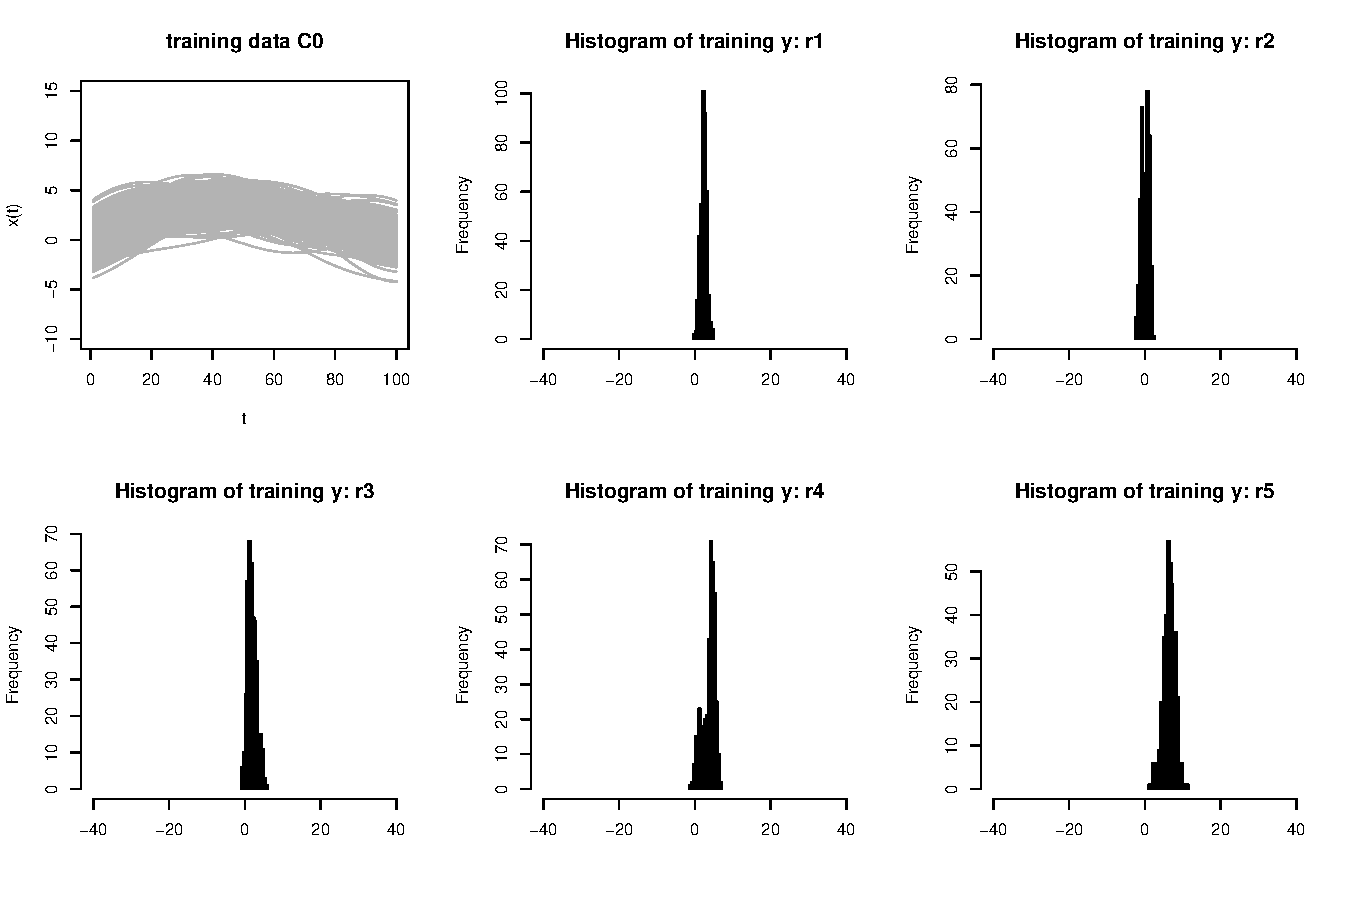
\includegraphics[scale = 0.55, page = 1]{figs/visualize_outliers.pdf}
\end{figure}

\begin{figure}[H]
    \centering
    \includegraphics[scale = 0.55, page = 2]{figs/visualize_outliers.pdf}
\end{figure}


\begin{figure}[H]
    \centering
    \includegraphics[scale = 0.55, page = 3]{figs/visualize_outliers.pdf}
\end{figure}


\begin{figure}[H]
    \centering
    \includegraphics[scale = 0.55, page = 4]{figs/visualize_outliers.pdf}
\end{figure}


\begin{figure}[H]
    \centering
    \includegraphics[scale = 0.55, page = 5]{figs/visualize_outliers.pdf}
\end{figure}

\begin{figure}[H]
    \centering
    \includegraphics[scale = 0.55, page = 6]{figs/visualize_outliers.pdf}
\end{figure}


\begin{figure}[H]
    \centering
    \includegraphics[scale = 0.55, page = 7]{figs/visualize_outliers.pdf}
\end{figure}

\begin{figure}[H]
    \centering5
    \includegraphics[scale = 0.55, page = 8]{figs/visualize_outliers.pdf}
\end{figure}


\subsection{Model comparison}
For each setting, we used 100 independently generated datasets and compared the performance of the following methods: 

\begin{itemize}
 \setlength\itemsep{0.1em}
\item \texttt{FPPR}: functional projection pursuit regression \citep{ferraty2013functional},
\item \texttt{FGAM}: functional generalized additive models \citep{mclean2014functional}, 
\item \texttt{MFLM}: Sieve M-estimator for a semi-functional linear model \citep{huang2015sieve},
\item \texttt{RFSIR}: robust functional sliced inverse regression \citep{wang2017robust}
\item \texttt{RFPLM}: robust estimation for semi-functional linear regression models \citep{boente2020robust},
\item  \texttt{TFBoost(L2)}:  tree-based functional boosting with L2 loss,
\item  \texttt{TFBoost(LAD)}:  tree-based functional boosting with LAD loss,
\item  \texttt{TFBoost(LAD-M)}:  tree-based functional boosting initialized with the robust residual scale estimators and function estimator obtained from \texttt{TFBoost(LAD)} followed by the second stage of \texttt{TFBoost(RR)}, 
\item  \texttt{TFBoost(RR.2)}:  proposed robust  tree-based functional boosting with $b = 0.2$, 
\item \texttt{TFBoost(RR.4)}:  proposed robust  tree-based functional boosting with $b = 0.4$, and
\item \texttt{TFBoost(RR.5)}:  proposed robust  tree-based functional boosting with $b = 0.5$ and initialized with multi-index LAD Tree. 
\end{itemize}

\subsection{Implementation details} \label{imp}

\begin{itemize}
	\item For \texttt{FPPR}, we implemented the method based on the code to fit a functional single index model shared by  the authors of \cite{ferraty2013functional}.  We used cubic B-spline with 7 functions (3 evenly spaced interior knots) as the basis and selected the number of additive components between 1 to 15 to minimize the validation  robust  MSPE, which is defined as
	$$\mu_M( \{y_i - \hat{F}(x_i)\}|i \in \mathcal{I}_{\text{val}})^2 + \hat{\sigma}_M(  \{y_i - \hat{F}(x_i)\}|i \in \mathcal{I}_{\text{val}}),$$
	where  $\hat{\mu}_M$ and $\hat{\sigma}_M$ are M-location and M-scale estimators specified to achieve 95\% asymptotic efficiency at the normal model. 
	\item For \texttt{FGAM},  we adopted the implementation in \texttt{refund} package. We set basis to be bivariate cubic B-splines of dimension 15 by 15 and used REML to select penalization parameter. 
	\item For \texttt{MFLM} and \texttt{RFPLM}, we adopted the implementation available from \\ https://github.com/msalibian/RobustFPLM. We considered cubic B-spline basis of dimension 4 to 7 with evenly spaced interior knots, and selected the dimension that minimized the BIC. 
	\item For \texttt{RFSIR}, we used the code shared by the author of \cite{wang2017robust}. We selected the number of leading functional principal components from 1 to 10 to minimize the validation  robust  MSPE. 
	\item For \texttt{TFBoost} methods  we used type B trees as base learners. With each training data, we selected the maximum depth of type B tree from 1 to 4 that achieves the lowest validation robust MSPE. 
	\item Considering that the first stage of \texttt{TFBoost(RR.5)} uses $b =  0.5$ which tends to treat individuals with large residuals as outliers compared to \texttt{TFBoost(RR)} with smaller $b$ values. 
	To avoid getting many zero gradients in early iterations and getting trapped in suboptima with poor objective values, we 
 initialize \texttt{TFBoost(RR.5)} with  Type A multi-index LADTrees. We set the minimum number of observations per node to be 10, fixed the number of indices $K = 1$, and selected the maximum depth of these trees from 0,1,2,3. 	
	
To  select the initial tree from 
    \begin{enumerate}
        \item[(a)] median of the training responses (depth 0 tree),
        \item[(b)] Type A tree with depth 1 and index 1,
        \item[(c)]  Type A tree with depth 2 and index 1, and
        \item[(d)] Type A tree with depth 3 and index 1,
    \end{enumerate}
    we follow the steps below. 
    \begin{itemize}
        \item Step 1: Fit \texttt{TFBoost(RR)} with (a) to obtain training and validation residuals $$r_{a,i} = \hat{F}_a(x_i) - y_i,$$
       and calculate M-scale of residuals (b = 0.5) for the training data and test data:
        $$M_{a, \text{train}}= \hat{\sigma}(r_{a,i}, i \in \mathcal{I}_{\text{train}})$$
    $$M_{a, \text{val}}= \hat{\sigma}(r_{a,i}, i \in \mathcal{I}_{\text{val}})$$
    \item Step 2: Flag outliers in the training data: 
    Let $\hat{\mu} = \text{median}(r_i, i \in \mathcal{I}_{\text{train}})$ and  $\hat{\sigma} = \text{MAD}(r_i, i \in \mathcal{I}_{\text{train}})$, the outliers are defined as
    $\mathcal{O}_a = \{i, i \in \mathcal{I}_{\text{train}}, |r_i - \hat{\mu}| > 3\hat{\sigma} \}$. 
        \item Step 3: Repeat Step 2 for \texttt{TFBoost(RR)} initialized with (b), (c), and (d), and denote the flagged outliers as  $\mathcal{O}_b$, $\mathcal{O}_c$, and $\mathcal{O}_d$ respectively.  Note that $\hat{\mu}$ and $\hat{\sigma}$ are calculated using \texttt{TFBoost(RR)} initialized with (a). 
        \item Step 4: Among (b), (c), (d), we only consider the ones that  ``fix" some outliers in $\mathcal{O}_a$. For example, (b) will be considered if some points in $\mathcal{O}_a$ are not in $\mathcal{O}_b$. 
        \item Step 5: For the  methods that passed the criterion in Step 4, we only consider the ones that have a lower validation residual scale compared to (a), and choose among them the one that 
        achieves the lowest training residual scale. 
        \item If no method remains after Step 5, we choose (a). 
    \end{itemize}
\end{itemize}


\subsection{Simulation results}
Below we report summary statistics of test MSPEs, displayed in the form of mean (sd) with the lowest two average test MPSEs bold-faced for each setting. 
\hspace{-2cm}
\renewcommand{\arraystretch}{1.5}
\addtolength{\tabcolsep}{-3pt} 

\newgeometry{left=1cm,bottom=0.1cm}
% material for this page
\subsubsection*{10\% outliers in training and validation sets}
% latex table generated in R 4.0.5 by xtable 1.8-4 package
% Mon Sep 13 00:10:42 2021
\begin{table}[H]
\centering
\begin{tabular}{rllllllll}
  \hline
 & $C_0$ & $C_1$ & $C_2$ & $C_3$ & $C_4$ & $C_5$ & $C_6$ & $C_7$ \\ 
  \hline
TFBoost(L2) & 0.14 (0.01) & 0.62 (0.39) & 0.91 (0.33) & 0.99 (0.37) & 1.24 (0.26) & 1.42 (0.84) & 11.24 (2.00) & 6.20 (1.87) \\ 
  TFBoost(LAD) & 0.15 (0.01) & 0.17 (0.05) & 0.19 (0.09) & 0.15 (0.01) & 0.19 (0.10) & 0.15 (0.01) & 0.16 (0.01) & 0.23 (0.17) \\ 
  TFBoost(LAD-M) & 0.15 (0.01) & 0.16 (0.04) & 0.17 (0.05) & 0.14 (0.01) & 0.17 (0.05) & 0.15 (0.01) & \textbf{0.15} (0.01) & 0.22 (0.17) \\ 
  TFBoost(RR.2) & 0.15 (0.01) & 0.15 (0.01) & \textbf{0.15} (0.01) & 0.14 (0.01) & 0.15 (0.01) & 0.15 (0.01) & \textbf{0.15} (0.01) & 0.15 (0.01) \\ 
  TFBoost(RR.4) & 0.15 (0.01) & 0.15 (0.01) & 0.16 (0.01) & 0.14 (0.01) & 0.15 (0.01) & 0.15 (0.01) & \textbf{0.15} (0.01) & 0.15 (0.01) \\ 
  TFBoost(RR.5) & 0.15 (0.01) & 0.15 (0.01) & 0.16 (0.01) & 0.14 (0.01) & 0.15 (0.01) & 0.15 (0.01) & \textbf{0.15} (0.01) & 0.15 (0.01) \\ 
  FPPR & 0.14 (0.01) & 3.06 (3.05) & 2.01 (2.84) & 6.60 (4.91) & 9.13 (5.03) & 2.68 (2.52) & 16.31 (4.85) & 0.74 (1.19) \\ 
  FGAM & \textbf{0.13} (0.01) & 3.03 (7.95) & 4.00 (7.02) & 44.49 (103.16) & 18.51 (49.94) & 0.91 (0.52) & 9.64 (0.60) & \textbf{0.13} (0.01) \\ 
  RFPLM & \textbf{0.13} (0.01) & \textbf{0.13} (0.01) & \textbf{0.13} (0.01) & \textbf{0.12} (0.00) & \textbf{0.13} (0.00) & \textbf{0.13} (0.01) & \textbf{0.13} (0.01) & \textbf{0.13} (0.01) \\ 
  MFLM & \textbf{0.13} (0.01) & \textbf{0.14} (0.01) & 0.20 (0.16) & \textbf{0.13} (0.01) & 0.17 (0.03) & \textbf{0.14} (0.01) & 0.34 (0.06) & \textbf{0.13} (0.01) \\ 
  RFSIR & 0.14 (0.01) & 0.94 (1.98) & 1.74 (2.65) & 0.14 (0.10) & \textbf{0.14} (0.01) & 1.14 (1.20) & 12.63 (4.23) & 0.19 (0.23) \\ 
   \hline
\end{tabular}
\caption{Summary statistics of test errors for data generated from $r_1$; displayed in the form of mean (sd).} 
\end{table}
% latex table generated in R 4.0.5 by xtable 1.8-4 package
% Mon Sep 13 00:10:42 2021
\begin{table}[H]
\centering
\begin{tabular}{rllllllll}
  \hline
 & $C_0$ & $C_1$ & $C_2$ & $C_3$ & $C_4$ & $C_5$ & $C_6$ & $C_7$ \\ 
  \hline
TFBoost(L2) & \textbf{0.18} (0.01) & 0.72 (0.37) & 1.02 (0.28) & 1.18 (0.29) & 1.49 (0.31) & 1.90 (1.02) & 11.56 (1.88) & 7.12 (1.27) \\ 
  TFBoost(LAD) & \textbf{0.18} (0.01) & 0.20 (0.07) & 0.22 (0.09) & 0.18 (0.01) & 0.24 (0.14) & \textbf{0.19} (0.01) & 0.20 (0.02) & 0.25 (0.09) \\ 
  TFBoost(LAD-M) & \textbf{0.18} (0.01) & 0.20 (0.04) & 0.21 (0.07) & 0.18 (0.02) & 0.23 (0.11) & \textbf{0.19} (0.01) & \textbf{0.19} (0.01) & 0.23 (0.08) \\ 
  TFBoost(RR.2) & \textbf{0.18} (0.01) & \textbf{0.18} (0.01) & \textbf{0.19} (0.01) & \textbf{0.17} (0.01) & \textbf{0.18} (0.01) & \textbf{0.18} (0.01) & \textbf{0.18} (0.01) & \textbf{0.18} (0.01) \\ 
  TFBoost(RR.4) & 0.19 (0.01) & \textbf{0.19} (0.01) & \textbf{0.19} (0.01) & \textbf{0.17} (0.01) & \textbf{0.18} (0.01) & \textbf{0.19} (0.01) & \textbf{0.19} (0.01) & \textbf{0.19} (0.01) \\ 
  TFBoost(RR.5) & 0.19 (0.01) & \textbf{0.19} (0.01) & \textbf{0.19} (0.01) & \textbf{0.17} (0.01) & \textbf{0.18} (0.01) & \textbf{0.19} (0.01) & \textbf{0.19} (0.01) & \textbf{0.19} (0.01) \\ 
  FPPR & \textbf{0.18} (0.01) & 3.34 (3.35) & 2.62 (2.68) & 6.79 (5.35) & 10.01 (4.48) & 2.76 (2.38) & 16.43 (4.73) & 1.03 (1.11) \\ 
  FGAM & 0.22 (0.01) & 3.13 (7.93) & 4.74 (8.23) & 42.13 (97.39) & 21.86 (63.03) & 1.04 (0.51) & 9.79 (0.60) & 0.23 (0.01) \\ 
  RFPLM & 0.29 (0.01) & 0.28 (0.01) & 0.29 (0.01) & 0.28 (0.01) & 0.29 (0.01) & 0.29 (0.01) & 0.29 (0.01) & 0.29 (0.01) \\ 
  MFLM & 0.28 (0.01) & 0.36 (0.15) & 0.54 (0.26) & 0.55 (0.16) & 0.70 (0.06) & 0.42 (0.17) & 0.83 (0.11) & 0.29 (0.01) \\ 
  RFSIR & \textbf{0.18} (0.01) & 1.37 (2.65) & 2.05 (3.32) & \textbf{0.17} (0.01) & 0.20 (0.07) & 1.54 (1.80) & 13.18 (5.36) & 0.24 (0.23) \\ 
   \hline
\end{tabular}
\caption{Summary statistics of test errors for data generated from $r_2$; displayed in the form of mean (sd).} 
\end{table}
% latex table generated in R 4.0.5 by xtable 1.8-4 package
% Mon Sep 13 00:10:42 2021
\begin{table}[H]
\centering
\begin{tabular}{rllllllll}
  \hline
 & $C_0$ & $C_1$ & $C_2$ & $C_3$ & $C_4$ & $C_5$ & $C_6$ & $C_7$ \\ 
  \hline
TFBoost(L2) & \textbf{0.31} (0.02) & 0.88 (0.49) & 1.52 (0.39) & 1.75 (0.32) & 2.07 (0.30) & 2.14 (1.18) & 11.73 (1.97) & 6.90 (1.82) \\ 
  TFBoost(LAD) & \textbf{0.31} (0.02) & 0.35 (0.09) & 0.35 (0.08) & 0.30 (0.02) & 0.38 (0.18) & \textbf{0.32} (0.02) & 0.34 (0.04) & 0.42 (0.14) \\ 
  TFBoost(LAD-M) & \textbf{0.31} (0.02) & 0.34 (0.06) & 0.34 (0.08) & 0.30 (0.01) & 0.34 (0.07) & \textbf{0.32} (0.02) & \textbf{0.32} (0.02) & 0.39 (0.12) \\ 
  TFBoost(RR.2) & 0.32 (0.03) & \textbf{0.32} (0.02) & \textbf{0.31} (0.02) & \textbf{0.29} (0.01) & \textbf{0.31} (0.01) & \textbf{0.31} (0.02) & \textbf{0.31} (0.02) & \textbf{0.32} (0.02) \\ 
  TFBoost(RR.4) & 0.32 (0.02) & \textbf{0.33} (0.04) & \textbf{0.32} (0.02) & 0.30 (0.01) & \textbf{0.32} (0.02) & \textbf{0.32} (0.03) & \textbf{0.32} (0.02) & 0.33 (0.03) \\ 
  TFBoost(RR.5) & 0.32 (0.02) & \textbf{0.33} (0.03) & \textbf{0.32} (0.02) & 0.30 (0.02) & \textbf{0.32} (0.02) & \textbf{0.32} (0.02) & \textbf{0.32} (0.02) & 0.33 (0.03) \\ 
  FPPR & \textbf{0.30} (0.02) & 3.22 (3.52) & 2.62 (2.70) & 6.45 (5.27) & 10.38 (4.75) & 2.60 (2.05) & 17.13 (5.04) & 1.26 (1.70) \\ 
  FGAM & 0.32 (0.01) & 3.20 (7.73) & 6.12 (15.06) & 39.73 (87.88) & 21.67 (58.30) & 1.15 (0.51) & 9.85 (0.58) & \textbf{0.32} (0.02) \\ 
  RFPLM & 0.38 (0.02) & 0.38 (0.02) & 0.38 (0.02) & 0.36 (0.01) & 0.38 (0.02) & 0.38 (0.02) & 0.38 (0.02) & 0.38 (0.02) \\ 
  MFLM & 0.38 (0.02) & 0.39 (0.03) & 0.53 (0.43) & 0.53 (0.47) & 2.53 (0.22) & 0.40 (0.03) & 1.39 (0.99) & 0.38 (0.02) \\ 
  RFSIR & \textbf{0.31} (0.02) & 1.73 (2.53) & 2.17 (3.04) & \textbf{0.29} (0.01) & 0.39 (0.64) & 1.26 (0.88) & 13.66 (4.77) & 0.39 (0.27) \\ 
   \hline
\end{tabular}
\caption{Summary statistics of test errors for data generated from $r_3$; displayed in the form of mean (sd).} 
\end{table}
% latex table generated in R 4.0.5 by xtable 1.8-4 package
% Mon Sep 13 00:10:43 2021
\begin{table}[H]
\centering
\begin{tabular}{rllllllll}
  \hline
 & $C_0$ & $C_1$ & $C_2$ & $C_3$ & $C_4$ & $C_5$ & $C_6$ & $C_7$ \\ 
  \hline
TFBoost(L2) & \textbf{0.52} (0.03) & 1.04 (0.48) & 2.20 (0.75) & 2.62 (0.35) & 2.96 (0.56) & 2.85 (1.30) & 12.35 (1.79) & 0.82 (0.22) \\ 
  TFBoost(LAD) & \textbf{0.53} (0.03) & 0.60 (0.13) & 0.61 (0.18) & 0.52 (0.03) & 0.68 (0.23) & 0.56 (0.05) & 0.55 (0.03) & 0.71 (0.26) \\ 
  TFBoost(LAD-M) & \textbf{0.53} (0.03) & 0.58 (0.11) & 0.57 (0.08) & \textbf{0.51} (0.03) & 0.64 (0.18) & \textbf{0.54} (0.03) & \textbf{0.54} (0.03) & 0.70 (0.26) \\ 
  TFBoost(RR.2) & 0.54 (0.05) & \textbf{0.55} (0.03) & \textbf{0.54} (0.03) & \textbf{0.50} (0.02) & \textbf{0.53} (0.03) & \textbf{0.53} (0.03) & \textbf{0.53} (0.03) & \textbf{0.54} (0.03) \\ 
  TFBoost(RR.4) & 0.54 (0.03) & \textbf{0.56} (0.04) & 0.56 (0.05) & 0.52 (0.03) & \textbf{0.54} (0.03) & 0.55 (0.04) & 0.55 (0.04) & \textbf{0.56} (0.04) \\ 
  TFBoost(RR.5) & 0.54 (0.03) & \textbf{0.56} (0.04) & \textbf{0.55} (0.04) & 0.52 (0.04) & \textbf{0.54} (0.03) & 0.55 (0.04) & 0.55 (0.04) & \textbf{0.56} (0.04) \\ 
  FPPR & 0.60 (0.05) & 4.30 (3.32) & 4.81 (3.44) & 9.05 (4.91) & 10.52 (5.25) & 4.24 (2.86) & 16.78 (4.52) & 1.49 (1.10) \\ 
  FGAM & 0.86 (0.04) & 3.86 (7.24) & 7.06 (11.76) & 34.52 (64.76) & 25.03 (67.45) & 2.23 (0.52) & 10.99 (0.71) & 0.87 (0.05) \\ 
  RFPLM & 1.11 (0.06) & 1.12 (0.08) & 1.12 (0.07) & 1.09 (0.06) & 1.11 (0.05) & 1.12 (0.06) & 1.12 (0.06) & 1.13 (0.10) \\ 
  MFLM & 1.10 (0.05) & 1.22 (0.18) & 1.34 (0.25) & 1.46 (0.19) & 1.72 (0.13) & 1.33 (0.22) & 1.94 (0.16) & 1.12 (0.07) \\ 
  RFSIR & 0.56 (0.04) & 2.17 (3.10) & 2.87 (3.78) & 0.54 (0.05) & 0.59 (0.13) & 2.38 (1.48) & 14.00 (5.62) & 0.61 (0.17) \\ 
   \hline
\end{tabular}
\caption{Summary statistics of test errors for data generated from $r_4$; displayed in the form of mean (sd).} 
\end{table}
% latex table generated in R 4.0.5 by xtable 1.8-4 package
% Mon Sep 13 00:10:43 2021
\begin{table}[H]
\centering
\begin{tabular}{rllllllll}
  \hline
 & $C_0$ & $C_1$ & $C_2$ & $C_3$ & $C_4$ & $C_5$ & $C_6$ & $C_7$ \\ 
  \hline
TFBoost(L2) & \textbf{0.58} (0.04) & 1.10 (0.49) & 2.19 (0.56) & 2.33 (0.27) & 2.62 (0.38) & 2.69 (1.05) & 12.50 (2.12) & 2.51 (2.26) \\ 
  TFBoost(LAD) & 0.61 (0.04) & 0.67 (0.11) & 0.69 (0.07) & 0.61 (0.04) & 0.68 (0.10) & 0.65 (0.05) & 0.65 (0.05) & 0.81 (0.27) \\ 
  TFBoost(LAD-M) & \textbf{0.60} (0.04) & \textbf{0.65} (0.10) & \textbf{0.66} (0.08) & \textbf{0.58} (0.04) & 0.69 (0.19) & \textbf{0.62} (0.05) & \textbf{0.62} (0.04) & 0.81 (0.25) \\ 
  TFBoost(RR.2) & 0.64 (0.06) & \textbf{0.61} (0.04) & \textbf{0.63} (0.04) & \textbf{0.58} (0.03) & \textbf{0.60} (0.03) & \textbf{0.61} (0.05) & \textbf{0.61} (0.04) & \textbf{0.60} (0.04) \\ 
  TFBoost(RR.4) & 0.66 (0.06) & 0.66 (0.06) & 0.69 (0.08) & 0.62 (0.06) & \textbf{0.65} (0.06) & 0.65 (0.07) & 0.67 (0.07) & 0.66 (0.07) \\ 
  TFBoost(RR.5) & 0.66 (0.07) & 0.66 (0.06) & 0.67 (0.07) & 0.62 (0.06) & \textbf{0.65} (0.06) & 0.66 (0.06) & 0.66 (0.06) & 0.65 (0.06) \\ 
  FPPR & 0.61 (0.06) & 4.15 (3.25) & 3.21 (2.61) & 7.99 (5.43) & 11.70 (5.34) & 3.50 (2.42) & 15.87 (4.70) & 1.24 (0.86) \\ 
  FGAM & \textbf{0.60} (0.04) & 3.73 (8.41) & 6.46 (10.95) & 33.73 (67.78) & 25.99 (82.71) & 1.90 (0.53) & 10.63 (0.73) & \textbf{0.60} (0.04) \\ 
  RFPLM & 0.88 (0.05) & 0.88 (0.05) & 0.88 (0.05) & 0.85 (0.05) & 0.89 (0.05) & 0.88 (0.05) & 0.88 (0.05) & 0.88 (0.05) \\ 
  MFLM & 0.87 (0.05) & 0.90 (0.05) & 1.02 (0.15) & 1.03 (0.43) & 1.85 (0.59) & 0.92 (0.07) & 1.99 (1.09) & 0.87 (0.04) \\ 
  RFSIR & 0.67 (0.06) & 2.08 (1.99) & 2.79 (3.05) & 0.70 (0.66) & 0.68 (0.20) & 2.14 (1.28) & 14.10 (4.84) & 0.72 (0.20) \\ 
   \hline
\end{tabular}
\caption{Summary statistics of test errors for data generated from $r_5$; displayed in the form of mean (sd).} 
\end{table}


\subsubsection*{30\% outliers in training and validation sets}
% latex table generated in R 4.0.5 by xtable 1.8-4 package
% Mon Sep 13 00:10:45 2021
\begin{table}[H]
\centering
\begin{tabular}{rllllllll}
  \hline
 & $C_0$ & $C_1$ & $C_2$ & $C_3$ & $C_4$ & $C_5$ & $C_6$ & $C_7$ \\ 
  \hline
TFBoost(L2) & 0.14 (0.01) & 0.96 (0.45) & 1.41 (0.79) & 1.10 (0.57) & 0.91 (0.17) & 2.78 (2.43) & 82.75 (2.00) & 69.67 (7.67) \\ 
  TFBoost(LAD) & 0.15 (0.01) & 0.20 (0.11) & 0.23 (0.15) & 0.17 (0.02) & 0.20 (0.16) & 0.17 (0.03) & 0.73 (2.33) & 0.74 (0.54) \\ 
  TFBoost(LAD-M) & 0.15 (0.01) & 0.18 (0.10) & 0.21 (0.14) & 0.16 (0.01) & 0.17 (0.11) & 0.16 (0.01) & 0.41 (1.33) & 0.62 (0.54) \\ 
  TFBoost(RR.2) & 0.15 (0.01) & 0.60 (0.47) & 0.30 (0.17) & 5.39 (3.43) & 1.19 (0.79) & 1.77 (1.95) & 45.94 (9.12) & 0.60 (0.35) \\ 
  TFBoost(RR.4) & 0.15 (0.01) & \textbf{0.16} (0.01) & \textbf{0.16} (0.01) & \textbf{0.15} (0.01) & \textbf{0.15} (0.01) & \textbf{0.15} (0.01) & \textbf{0.15} (0.01) & 0.16 (0.01) \\ 
  TFBoost(RR.5) & 0.15 (0.01) & \textbf{0.16} (0.01) & 0.17 (0.02) & \textbf{0.15} (0.01) & \textbf{0.15} (0.01) & \textbf{0.15} (0.01) & \textbf{0.15} (0.01) & 0.16 (0.01) \\ 
  FPPR & 0.14 (0.01) & 2.67 (2.77) & 0.96 (1.07) & 16.57 (11.51) & 11.73 (8.08) & 6.86 (6.42) & 109.00 (16.52) & 0.76 (1.00) \\ 
  FGAM & \textbf{0.13} (0.01) & 1.21 (0.82) & 1.17 (1.00) & 5.16 (2.86) & 2.32 (1.31) & 2.44 (2.10) & 82.17 (1.54) & \textbf{0.13} (0.01) \\ 
  RFPLM & \textbf{0.13} (0.01) & \textbf{0.13} (0.01) & \textbf{0.13} (0.01) & \textbf{0.13} (0.00) & \textbf{0.13} (0.00) & \textbf{0.13} (0.01) & \textbf{0.13} (0.01) & \textbf{0.13} (0.01) \\ 
  MFLM & \textbf{0.13} (0.01) & 0.24 (0.16) & 0.56 (0.48) & 0.24 (0.13) & 0.42 (0.23) & 0.22 (0.12) & 23.38 (2.91) & \textbf{0.13} (0.01) \\ 
  RFSIR & 0.14 (0.01) & 1.27 (2.61) & 1.14 (2.08) & 0.16 (0.03) & 0.27 (0.19) & 2.03 (2.32) & 87.49 (7.31) & 0.29 (0.46) \\ 
   \hline
\end{tabular}
\caption{Summary statistics of test errors for data generated from $r_1$; displayed in the form of mean (sd).} 
\end{table}
% latex table generated in R 4.0.5 by xtable 1.8-4 package
% Mon Sep 13 00:10:45 2021
\begin{table}[H]
\centering
\begin{tabular}{rllllllll}
  \hline
 & $C_0$ & $C_1$ & $C_2$ & $C_3$ & $C_4$ & $C_5$ & $C_6$ & $C_7$ \\ 
  \hline
TFBoost(L2) & \textbf{0.18} (0.01) & 1.10 (0.55) & 1.28 (0.48) & 1.36 (0.62) & 1.11 (0.13) & 3.01 (2.18) & 83.09 (2.18) & 63.85 (7.28) \\ 
  TFBoost(LAD) & \textbf{0.18} (0.01) & 0.25 (0.18) & 0.27 (0.15) & 0.22 (0.07) & 0.23 (0.24) & 0.20 (0.01) & 0.79 (2.27) & 0.56 (0.42) \\ 
  TFBoost(LAD-M) & \textbf{0.18} (0.01) & 0.21 (0.06) & 0.24 (0.11) & 0.21 (0.07) & 0.21 (0.19) & \textbf{0.19} (0.01) & 0.73 (2.53) & 0.35 (0.36) \\ 
  TFBoost(RR.2) & \textbf{0.18} (0.01) & 0.74 (0.66) & 0.41 (0.27) & 5.30 (3.50) & 1.18 (0.74) & 1.88 (1.85) & 46.15 (8.02) & 1.49 (0.27) \\ 
  TFBoost(RR.4) & 0.19 (0.01) & \textbf{0.19} (0.01) & \textbf{0.19} (0.01) & \textbf{0.19} (0.01) & \textbf{0.18} (0.01) & \textbf{0.18} (0.01) & \textbf{0.19} (0.01) & \textbf{0.21} (0.01) \\ 
  TFBoost(RR.5) & 0.19 (0.01) & \textbf{0.19} (0.01) & \textbf{0.19} (0.01) & \textbf{0.19} (0.01) & \textbf{0.18} (0.01) & \textbf{0.19} (0.01) & \textbf{0.19} (0.01) & \textbf{0.21} (0.02) \\ 
  FPPR & \textbf{0.18} (0.01) & 3.44 (3.39) & 2.21 (3.04) & 19.06 (12.71) & 11.95 (6.73) & 7.44 (6.88) & 104.41 (15.89) & 1.19 (1.49) \\ 
  FGAM & 0.22 (0.01) & 1.33 (0.83) & 1.35 (0.95) & 5.26 (2.84) & 2.27 (1.11) & 2.60 (2.11) & 82.34 (1.60) & 0.23 (0.01) \\ 
  RFPLM & 0.29 (0.01) & 0.29 (0.01) & 0.33 (0.03) & 0.29 (0.01) & 0.29 (0.01) & 0.29 (0.01) & 0.29 (0.01) & 0.31 (0.02) \\ 
  MFLM & 0.28 (0.01) & 0.73 (0.22) & 1.02 (0.51) & 0.72 (0.27) & 0.95 (0.24) & 0.77 (0.17) & 23.57 (2.90) & 0.31 (0.01) \\ 
  RFSIR & \textbf{0.18} (0.01) & 1.63 (2.75) & 1.51 (2.61) & 0.22 (0.19) & 0.47 (1.09) & 2.09 (2.32) & 86.15 (5.78) & 0.29 (0.30) \\ 
   \hline
\end{tabular}
\caption{Summary statistics of test errors for data generated from $r_2$; displayed in the form of mean (sd).} 
\end{table}
% latex table generated in R 4.0.5 by xtable 1.8-4 package
% Mon Sep 13 00:10:45 2021
\begin{table}[H]
\centering
\begin{tabular}{rllllllll}
  \hline
 & $C_0$ & $C_1$ & $C_2$ & $C_3$ & $C_4$ & $C_5$ & $C_6$ & $C_7$ \\ 
  \hline
TFBoost(L2) & \textbf{0.31} (0.02) & 1.43 (0.60) & 1.84 (0.51) & 1.99 (0.62) & 1.68 (0.15) & 3.37 (2.43) & 83.09 (2.10) & 66.47 (7.74) \\ 
  TFBoost(LAD) & \textbf{0.31} (0.02) & 0.40 (0.12) & 0.40 (0.11) & 0.37 (0.04) & 0.38 (0.17) & 0.35 (0.04) & 1.22 (2.96) & 0.92 (0.51) \\ 
  TFBoost(LAD-M) & \textbf{0.31} (0.02) & 0.37 (0.10) & 0.37 (0.13) & \textbf{0.33} (0.03) & 0.35 (0.15) & \textbf{0.33} (0.02) & 0.91 (2.82) & 0.79 (0.48) \\ 
  TFBoost(RR.2) & 0.32 (0.03) & 0.79 (0.45) & 0.58 (0.29) & 5.84 (3.62) & 1.43 (0.83) & 2.53 (2.48) & 45.84 (8.25) & 1.10 (0.67) \\ 
  TFBoost(RR.4) & 0.32 (0.02) & \textbf{0.34} (0.02) & \textbf{0.32} (0.02) & \textbf{0.32} (0.01) & \textbf{0.31} (0.01) & \textbf{0.32} (0.02) & \textbf{0.32} (0.02) & \textbf{0.34} (0.02) \\ 
  TFBoost(RR.5) & 0.32 (0.02) & \textbf{0.34} (0.02) & \textbf{0.33} (0.02) & \textbf{0.33} (0.02) & \textbf{0.31} (0.02) & \textbf{0.33} (0.02) & \textbf{0.33} (0.02) & 0.35 (0.03) \\ 
  FPPR & \textbf{0.30} (0.02) & 3.97 (4.23) & 2.90 (3.74) & 18.64 (10.91) & 11.70 (7.08) & 6.78 (6.71) & 108.99 (18.23) & 1.28 (1.39) \\ 
  FGAM & 0.32 (0.01) & 1.49 (0.88) & 1.55 (0.89) & 5.31 (2.86) & 2.55 (1.24) & 2.70 (2.10) & 82.39 (1.68) & \textbf{0.33} (0.02) \\ 
  RFPLM & 0.38 (0.02) & 0.38 (0.02) & 0.43 (0.05) & 0.39 (0.02) & 0.37 (0.02) & 0.38 (0.02) & 0.38 (0.02) & 0.40 (0.02) \\ 
  MFLM & 0.38 (0.02) & 0.69 (0.66) & 1.33 (1.13) & 0.58 (0.19) & 3.04 (0.41) & 0.92 (0.95) & 25.24 (2.92) & 0.39 (0.02) \\ 
  RFSIR & \textbf{0.31} (0.02) & 1.36 (1.32) & 1.60 (1.52) & 0.36 (0.30) & 0.44 (0.26) & 2.49 (2.30) & 86.70 (7.06) & 0.47 (0.37) \\ 
   \hline
\end{tabular}
\caption{Summary statistics of test errors for data generated from $r_3$; displayed in the form of mean (sd).} 
\end{table}
% latex table generated in R 4.0.5 by xtable 1.8-4 package
% Mon Sep 13 00:10:46 2021
\begin{table}[H]
\centering
\begin{tabular}{rllllllll}
  \hline
 & $C_0$ & $C_1$ & $C_2$ & $C_3$ & $C_4$ & $C_5$ & $C_6$ & $C_7$ \\ 
  \hline
TFBoost(L2) & \textbf{0.52} (0.03) & 1.68 (0.65) & 2.62 (0.51) & 3.03 (0.80) & 2.75 (0.22) & 4.40 (2.66) & 84.01 (2.36) & 1.11 (0.36) \\ 
  TFBoost(LAD) & \textbf{0.53} (0.03) & 0.74 (0.23) & 0.70 (0.19) & 0.67 (0.10) & 0.70 (0.21) & 0.62 (0.12) & 1.23 (2.40) & 1.25 (0.60) \\ 
  TFBoost(LAD-M) & \textbf{0.53} (0.03) & 0.66 (0.14) & 0.66 (0.19) & 0.61 (0.09) & 0.60 (0.20) & 0.58 (0.04) & 0.95 (2.22) & 1.19 (0.55) \\ 
  TFBoost(RR.2) & 0.54 (0.05) & 1.53 (0.90) & 0.85 (0.37) & 6.45 (2.98) & 2.01 (1.04) & 3.64 (2.21) & 46.12 (9.48) & 0.97 (0.32) \\ 
  TFBoost(RR.4) & 0.54 (0.03) & \textbf{0.61} (0.04) & \textbf{0.58} (0.04) & \textbf{0.56} (0.03) & \textbf{0.54} (0.04) & \textbf{0.55} (0.04) & \textbf{0.55} (0.03) & \textbf{0.58} (0.03) \\ 
  TFBoost(RR.5) & 0.54 (0.03) & \textbf{0.60} (0.04) & \textbf{0.59} (0.04) & \textbf{0.57} (0.03) & \textbf{0.54} (0.03) & \textbf{0.57} (0.04) & \textbf{0.56} (0.04) & \textbf{0.59} (0.03) \\ 
  FPPR & 0.60 (0.05) & 4.11 (3.06) & 3.87 (2.92) & 17.87 (10.62) & 14.34 (7.78) & 8.36 (6.19) & 105.62 (15.95) & 2.07 (1.64) \\ 
  FGAM & 0.86 (0.04) & 2.47 (0.86) & 2.53 (0.89) & 6.17 (3.01) & 4.11 (1.65) & 3.88 (2.18) & 83.56 (2.01) & 0.90 (0.05) \\ 
  RFPLM & 1.11 (0.06) & 1.14 (0.06) & 1.16 (0.07) & 1.13 (0.06) & 1.13 (0.07) & 1.11 (0.06) & 1.11 (0.06) & 1.25 (0.12) \\ 
  MFLM & 1.10 (0.05) & 1.69 (0.26) & 1.97 (0.79) & 1.73 (0.38) & 2.11 (0.40) & 1.76 (0.26) & 24.63 (2.94) & 1.22 (0.08) \\ 
  RFSIR & 0.56 (0.04) & 1.70 (1.55) & 2.70 (2.32) & 0.86 (1.77) & 0.91 (0.59) & 3.68 (2.47) & 87.10 (7.16) & 0.65 (0.25) \\ 
   \hline
\end{tabular}
\caption{Summary statistics of test errors for data generated from $r_4$; displayed in the form of mean (sd).} 
\end{table}
% latex table generated in R 4.0.5 by xtable 1.8-4 package
% Mon Sep 13 00:10:46 2021
\begin{table}[H]
\centering
\begin{tabular}{rllllllll}
  \hline
 & $C_0$ & $C_1$ & $C_2$ & $C_3$ & $C_4$ & $C_5$ & $C_6$ & $C_7$ \\ 
  \hline
TFBoost(L2) & \textbf{0.58} (0.04) & 1.74 (0.60) & 2.63 (0.86) & 2.44 (0.53) & 2.32 (0.20) & 3.87 (1.79) & 84.07 (2.27) & 68.34 (7.96) \\ 
  TFBoost(LAD) & 0.61 (0.04) & 0.72 (0.09) & 0.82 (0.23) & 0.77 (0.07) & 0.79 (0.27) & 0.75 (0.07) & 1.41 (1.33) & 1.45 (0.65) \\ 
  TFBoost(LAD-M) & \textbf{0.60} (0.04) & \textbf{0.67} (0.07) & 0.74 (0.21) & 0.68 (0.10) & 0.70 (0.25) & \textbf{0.67} (0.05) & 1.27 (2.81) & 1.32 (0.57) \\ 
  TFBoost(RR.2) & 0.64 (0.06) & 1.24 (0.58) & 0.91 (0.23) & 6.02 (2.78) & 1.75 (0.77) & 3.15 (2.03) & 45.84 (8.63) & 1.04 (0.35) \\ 
  TFBoost(RR.4) & 0.66 (0.06) & \textbf{0.65} (0.05) & \textbf{0.70} (0.05) & \textbf{0.65} (0.05) & \textbf{0.64} (0.04) & \textbf{0.65} (0.04) & \textbf{0.64} (0.04) & \textbf{0.64} (0.04) \\ 
  TFBoost(RR.5) & 0.66 (0.07) & \textbf{0.67} (0.06) & \textbf{0.72} (0.05) & \textbf{0.67} (0.06) & \textbf{0.65} (0.05) & \textbf{0.67} (0.06) & \textbf{0.67} (0.06) & 0.67 (0.06) \\ 
  FPPR & 0.61 (0.06) & 4.00 (3.80) & 2.59 (1.62) & 17.34 (10.58) & 12.88 (6.91) & 7.94 (6.12) & 106.34 (14.44) & 1.58 (1.10) \\ 
  FGAM & \textbf{0.60} (0.04) & 2.17 (0.78) & 2.11 (0.88) & 5.76 (2.89) & 3.35 (1.42) & 3.48 (2.05) & 83.32 (1.95) & \textbf{0.62} (0.04) \\ 
  RFPLM & 0.88 (0.05) & 0.88 (0.04) & 0.97 (0.06) & 0.89 (0.05) & 0.90 (0.05) & 0.88 (0.05) & 0.88 (0.05) & 0.89 (0.04) \\ 
  MFLM & 0.87 (0.05) & 1.22 (0.63) & 1.70 (1.00) & 1.15 (0.23) & 3.84 (0.48) & 1.47 (1.00) & 26.11 (2.88) & 0.91 (0.05) \\ 
  RFSIR & 0.67 (0.06) & 1.92 (1.78) & 2.41 (2.22) & 0.73 (0.27) & 1.09 (0.95) & 3.23 (2.42) & 86.80 (6.65) & 0.84 (0.34) \\ 
   \hline
\end{tabular}
\caption{Summary statistics of test errors for data generated from $r_5$; displayed in the form of mean (sd).} 
\end{table}


\restoregeometry

\section{Real example} 
We analyze the fruit fly data available at https://anson.ucdavis.edu/~mueller/data/data.html. The data set  consists of number of eggs laid daily for each of 1000 medflies  until time of death. We used a subset of the data including flies that lived at least 30 days, to predict the number of living days. The number of eggs laid in the first 30 days is treated as the functional predictor with values evaluated at each day. 

We randomly portioned the data into 60\% training set, 20\% validation set, and 20\% test set.  The description and set-ups of all methods follows the details in \Cref{imp}. Since the test set may contain outliers,  average absolute values (AAD) of the residuals on the test set are used for comparison.  To avoid randomness introduced by a single partition, we considered 100 random partitions. The summary statistics of test robust MSPEs are shown in \Cref{fig:ori}.  To be able to see the differences, the TFBoost methods are plotted separately from the other methods. 

\begin{figure}
	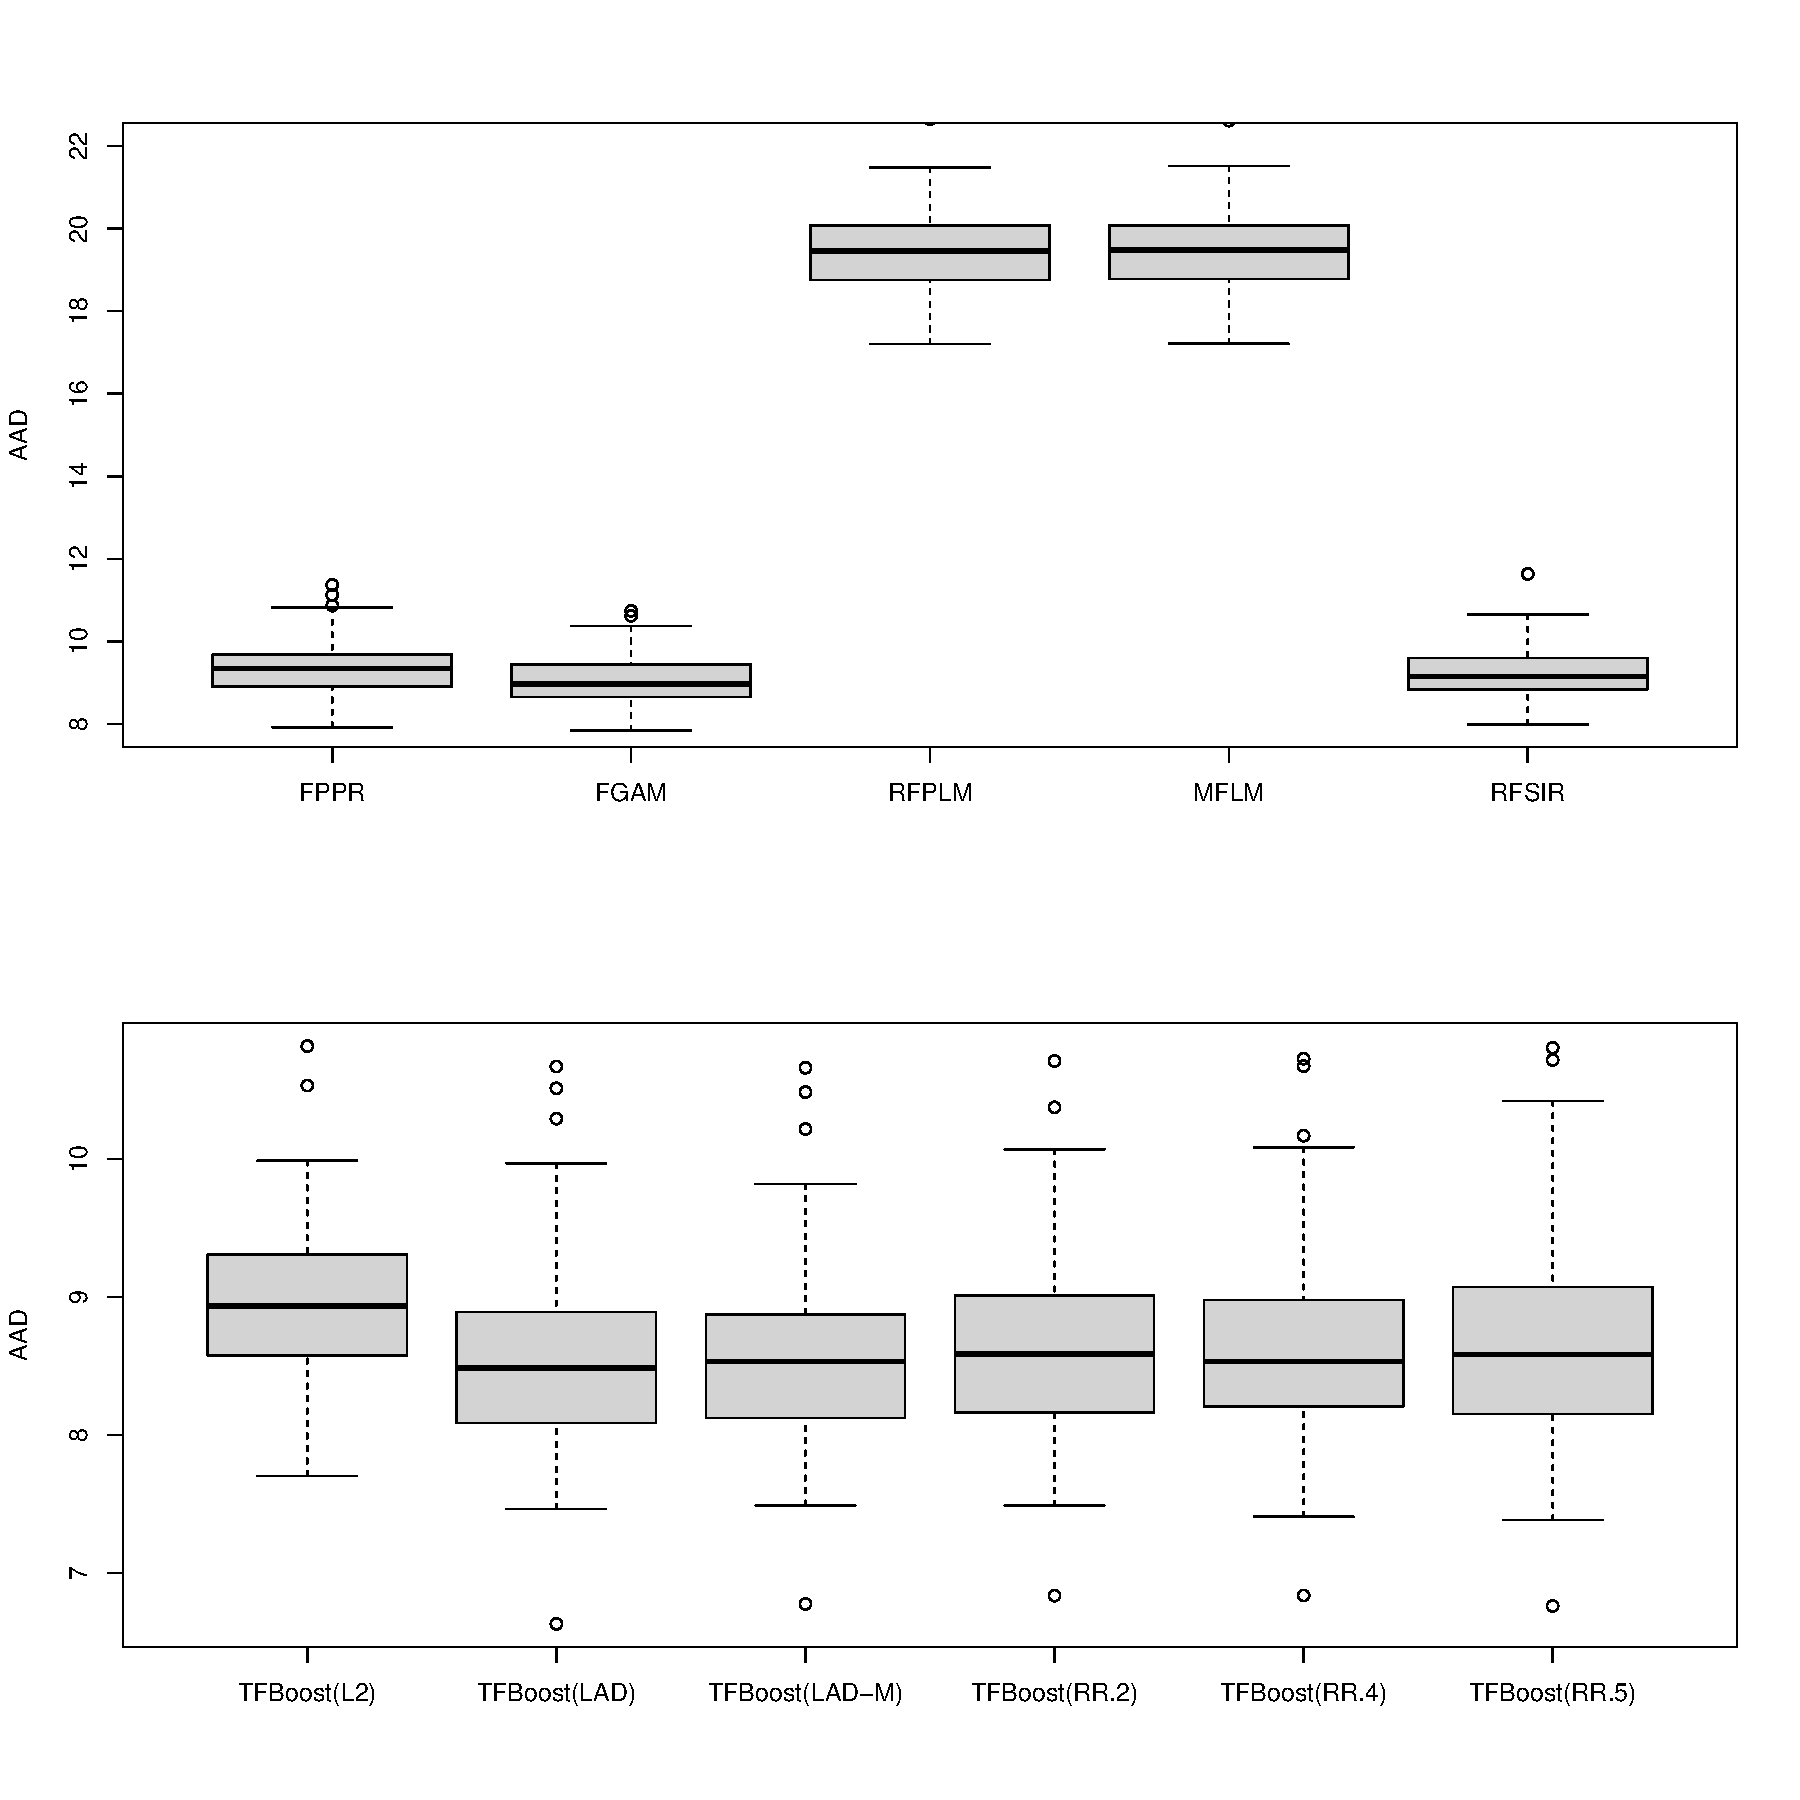
\includegraphics[scale = 0.5]{figs/Frui_Fly.pdf}
	\caption{Test AADs  obtained from 100 random partitions of the FruitFly data}
	\label{fig:ori}
\end{figure}


To further illustrate the performance of our method when data contain more extreme outliers. We considered adding symmetric and asymmetric outliers to the responses in the training and the validation sets. We randomly sample 20\% of the individuals (denoted as $\mathcal{O}$), and let there responses be 
$$\tilde{y}_{i} = y_i + \eta_i, i \in \mathcal{I}$$ 
where $y_i$ is the original response, and $\eta_i \ = \text{round}(e_i)$, where $e_i \sim 0.5N(30, 3) + 0.5N(-30, 3)$ for symmetric outliers and $e_i \sim N(30, 3)$ for asymmetric outliers. The robust MSPEs from 100 random partitions of the data are shown below. 

\begin{figure}
	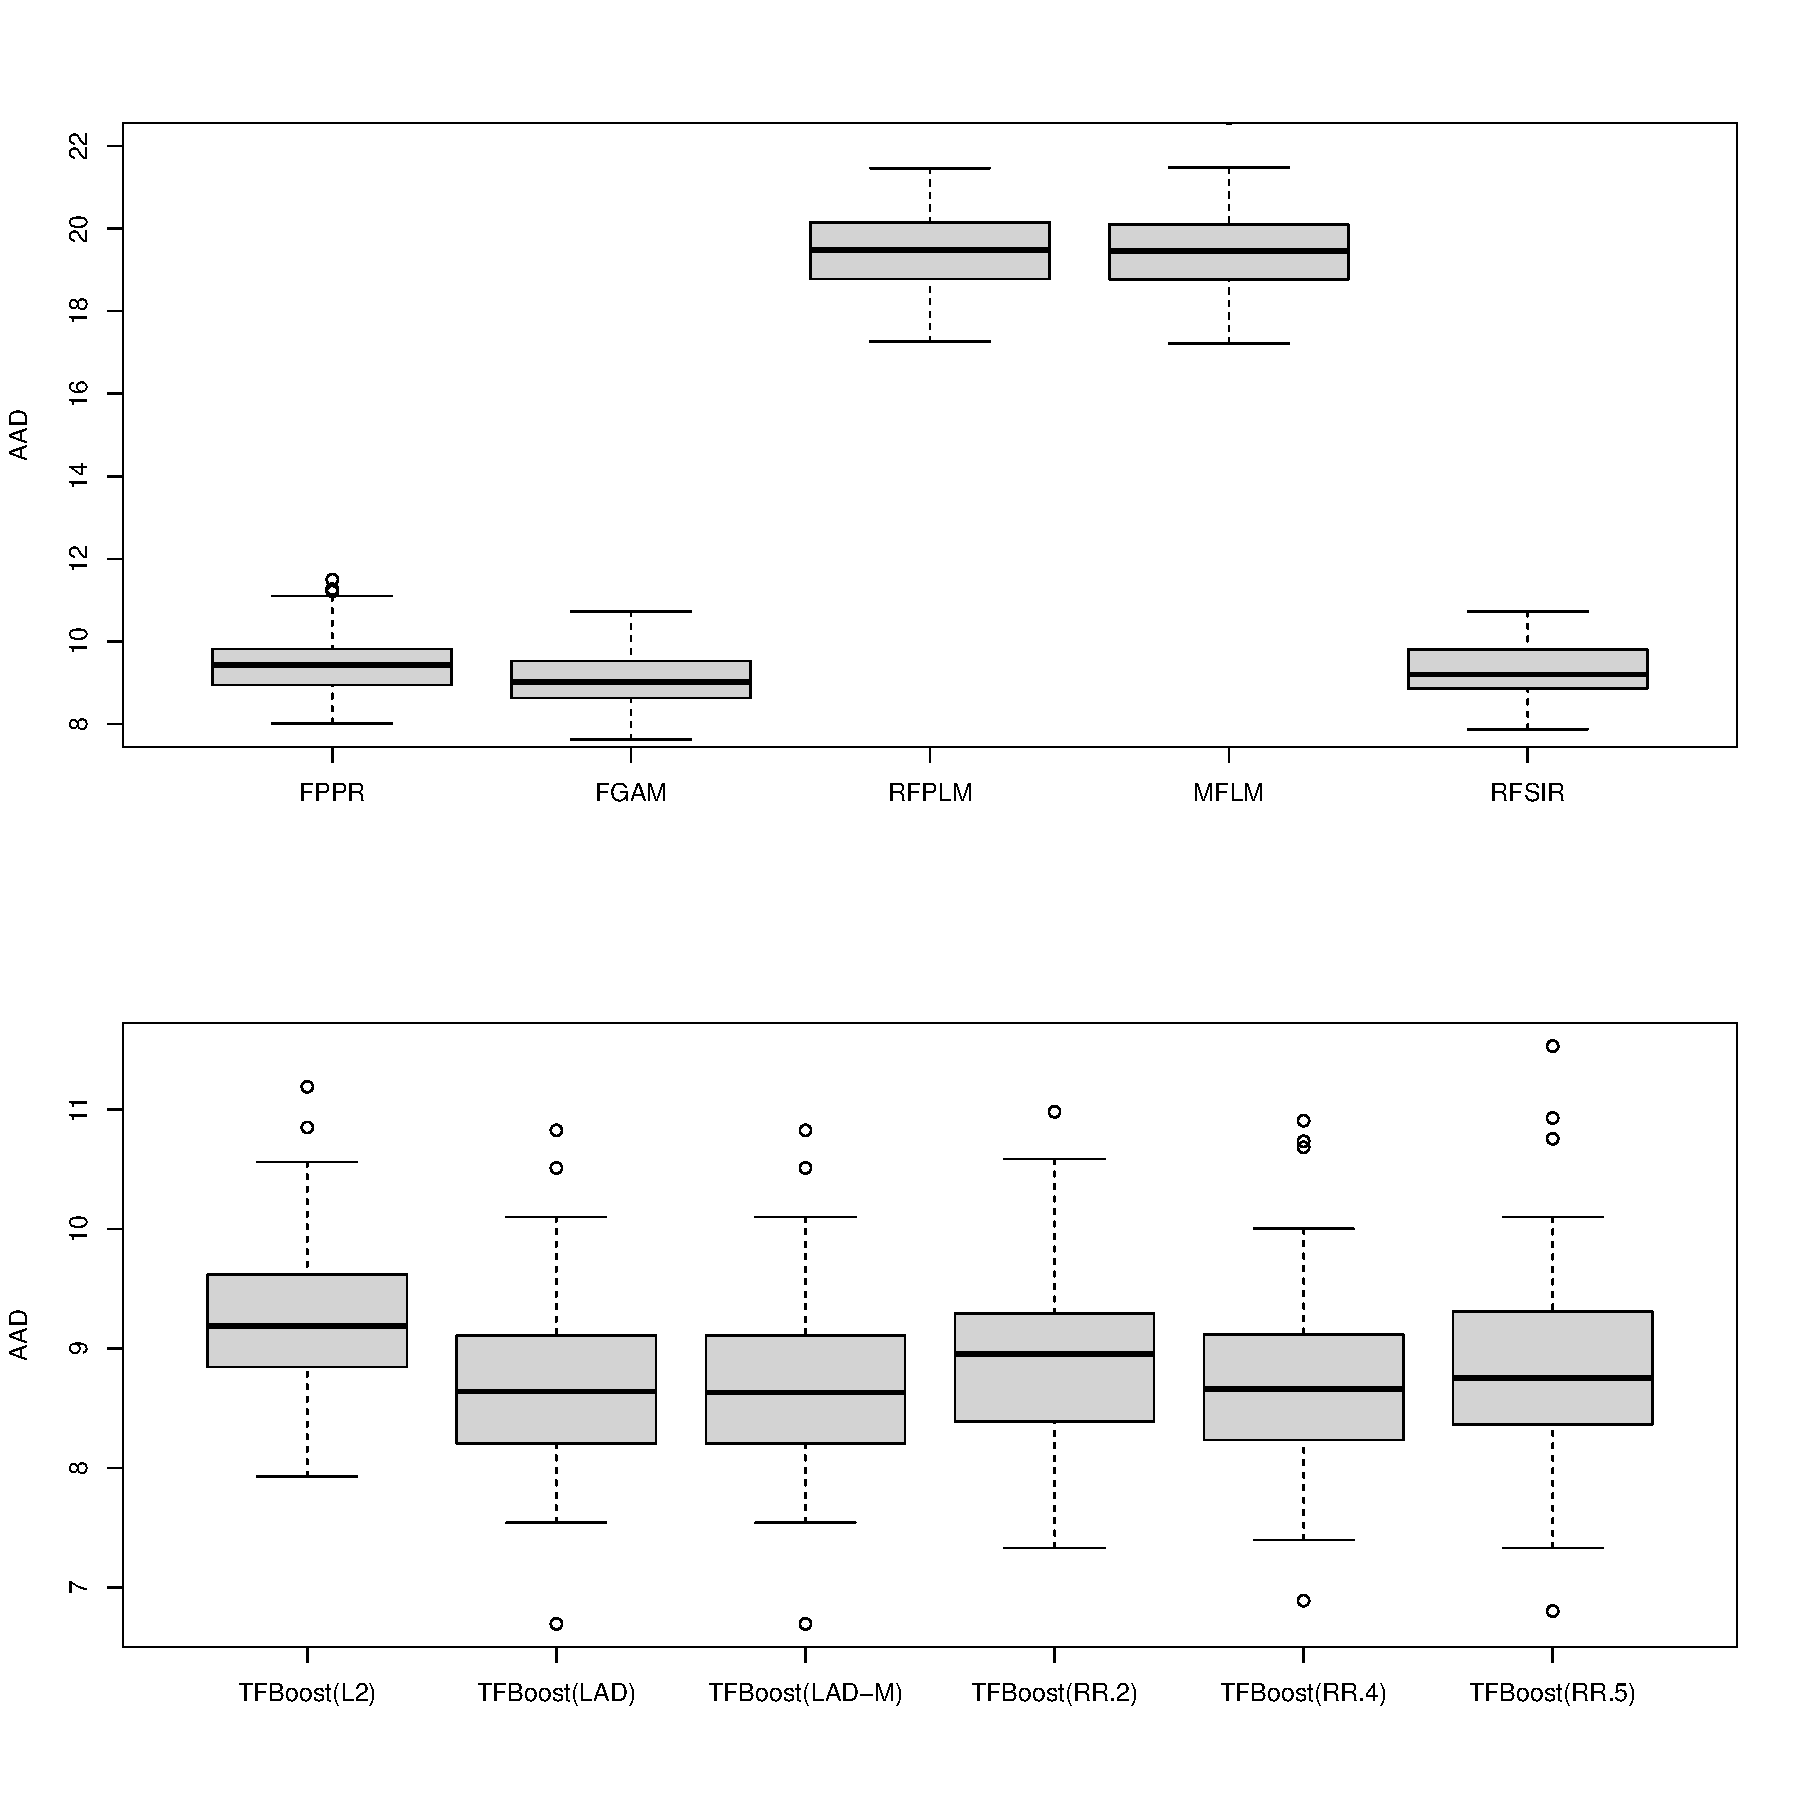
\includegraphics[scale = 0.5]{figs/Frui_Fly_B.pdf}
	\caption{Test AADs obtained from 100 random partitions of the FruitFly data with symmetric outliers}
\end{figure}


\begin{figure}
	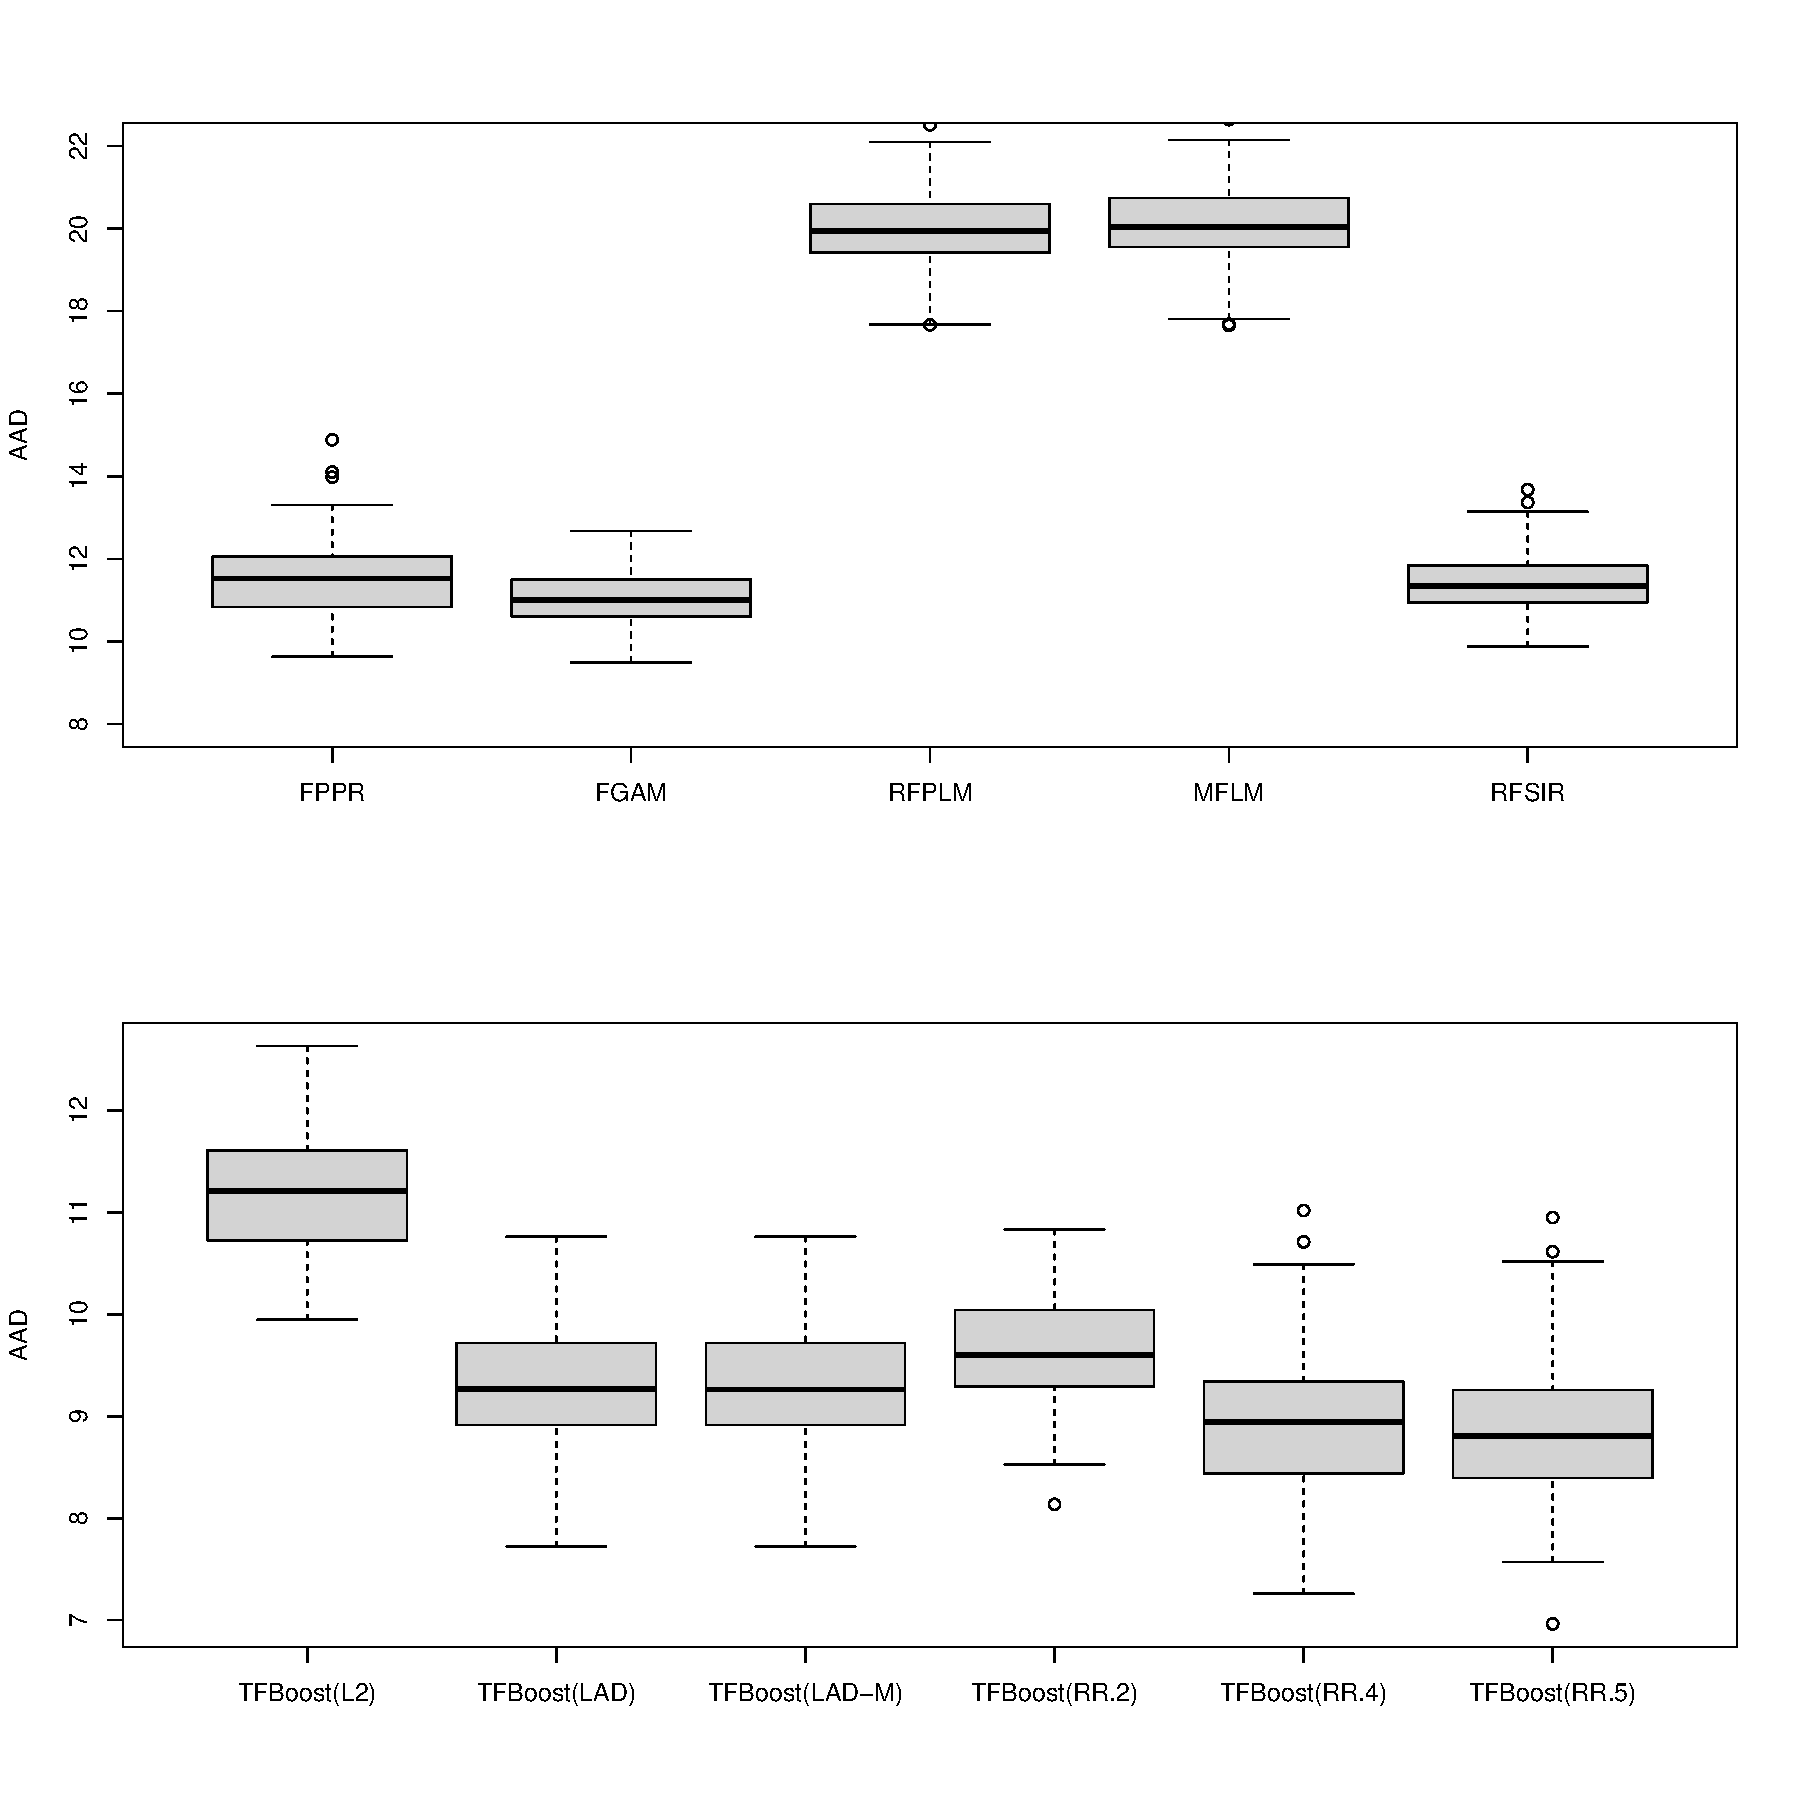
\includegraphics[scale = 0.5]{figs/Frui_Fly_A.pdf}
	\caption{Test AADs  obtained from 100 random partitions of the FruitFly data with asymmetric outliers}
\end{figure}




%Summary statistics of test MSPEs, displayed in the form of mean (sd). 
%\texttt{TFBoost(RR.5)} and \texttt{TFBoost(RR.2)} were initialized with the \texttt{LADTrees} with the maximum depth chosen from $\{0,1,2,3\}$ and the minimum number of observations per node chosen from 
%$\{10,20,30\}$. 
%
\bibliographystyle{apalike}
\bibliography{reference}
\end{document}
